% Created 2021-03-18 Thu 11:29
% Intended LaTeX compiler: pdflatex

\documentclass[english]{article}
\usepackage[T1, T2A]{fontenc}
\usepackage[lutf8]{luainputenc}
\usepackage[english, russian]{babel}
\usepackage{minted}
\usepackage{graphicx}
\usepackage{longtable}
\usepackage{hyperref}
\usepackage{xcolor}
\usepackage{natbib}
\usepackage{amssymb}
\usepackage{stmaryrd}
\usepackage{amsmath}
\usepackage{caption}
\usepackage{mathtools}
\usepackage{amsthm}
\usepackage{tikz}
\usepackage{grffile}
\usepackage{extarrows}
\usepackage{wrapfig}
\usepackage{rotating}
\usepackage{placeins}
\usepackage[normalem]{ulem}
\usepackage{amsmath}
\usepackage{textcomp}
\usepackage{capt-of}

\usepackage{geometry}
\geometry{a4paper,left=2.5cm,top=2cm,right=2.5cm,bottom=2cm,marginparsep=7pt, marginparwidth=.6in}

 \usepackage{hyperref}
 \hypersetup{
     colorlinks=true,
     linkcolor=blue,
     filecolor=orange,
     citecolor=black,      
     urlcolor=cyan,
     }

\usetikzlibrary{decorations.markings}
\usetikzlibrary{cd}
\usetikzlibrary{patterns}
\usetikzlibrary{automata, arrows}

\newcommand\addtag{\refstepcounter{equation}\tag{\theequation}}
\newcommand{\eqrefoffset}[1]{\addtocounter{equation}{-#1}(\arabic{equation}\addtocounter{equation}{#1})}


\newcommand{\R}{\mathbb{R}}
\renewcommand{\C}{\mathbb{C}}
\newcommand{\N}{\mathbb{N}}
\newcommand{\rank}{\text{rank}}
\newcommand{\const}{\text{const}}
\newcommand{\grad}{\text{grad}}

\theoremstyle{plain}
\newtheorem{axiom}{Аксиома}
\newtheorem{lemma}{Лемма}
\newtheorem{manuallemmainner}{Лемма}
\newenvironment{manuallemma}[1]{%
  \renewcommand\themanuallemmainner{#1}%
  \manuallemmainner
}{\endmanuallemmainner}

\theoremstyle{remark}
\newtheorem*{remark}{Примечание}
\newtheorem*{solution}{Решение}
\newtheorem{corollary}{Следствие}[theorem]
\newtheorem*{examp}{Пример}
\newtheorem*{observation}{Наблюдение}

\theoremstyle{definition}
\newtheorem{task}{Задача}
\newtheorem{theorem}{Теорема}[section]
\newtheorem*{definition}{Определение}
\newtheorem*{symb}{Обозначение}
\newtheorem{manualtheoreminner}{Теорема}
\newenvironment{manualtheorem}[1]{%
  \renewcommand\themanualtheoreminner{#1}%
  \manualtheoreminner
}{\endmanualtheoreminner}
\captionsetup{justification=centering,margin=2cm}
\newenvironment{colored}[1]{\color{#1}}{}

\tikzset{->-/.style={decoration={
  markings,
  mark=at position .5 with {\arrow{>}}},postaction={decorate}}}
\makeatletter
\newcommand*{\relrelbarsep}{.386ex}
\newcommand*{\relrelbar}{%
  \mathrel{%
    \mathpalette\@relrelbar\relrelbarsep
  }%
}
\newcommand*{\@relrelbar}[2]{%
  \raise#2\hbox to 0pt{$\m@th#1\relbar$\hss}%
  \lower#2\hbox{$\m@th#1\relbar$}%
}
\providecommand*{\rightrightarrowsfill@}{%
  \arrowfill@\relrelbar\relrelbar\rightrightarrows
}
\providecommand*{\leftleftarrowsfill@}{%
  \arrowfill@\leftleftarrows\relrelbar\relrelbar
}
\providecommand*{\xrightrightarrows}[2][]{%
  \ext@arrow 0359\rightrightarrowsfill@{#1}{#2}%
}
\providecommand*{\xleftleftarrows}[2][]{%
  \ext@arrow 3095\leftleftarrowsfill@{#1}{#2}%
}
\makeatother
\author{Ilya Yaroshevskiy}
\date{\today}
\title{Практика 6}
\hypersetup{
 pdfauthor={Ilya Yaroshevskiy},
 pdftitle={Практика 6},
 pdfkeywords={},
 pdfsubject={},
 pdfcreator={Emacs 28.0.50 (Org mode )}, 
 pdflang={English}}
\begin{document}

\maketitle
\tableofcontents

\begin{task}
\[ \int_\Omega \frac{1}{|x + y|^p} dx dy \]
\begin{center}
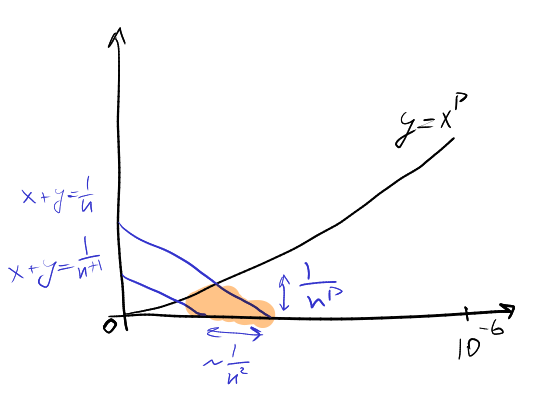
\includegraphics[scale=0.5]{6_1.png}
\end{center}
\end{task}
\begin{solution}
\[ \int_\Omega \frac{1}{|x + y|^p} dx dy = \sum_n \int_{\Omega_n} \asymp \sum_n \frac{1}{\left(\frac{1}{n}\right)^p}\cdot \frac{1}{n^{p + 2}} \]
\end{solution}
\begin{task}
Тоже самое с четвертинкой астроиды
\end{task}
\begin{solution}
\[ \int_\Omega \frac{1}{|x + y|^p} dx dy \asymp \sum \frac{1}{n^{3 - p}} \]
\end{solution}
\begin{task}
\[ \int_\Omega \frac{1}{|1 - x^2 - y^2|} dx dy \],
\(\Omega\) --- четверть астроиды
\begin{center}
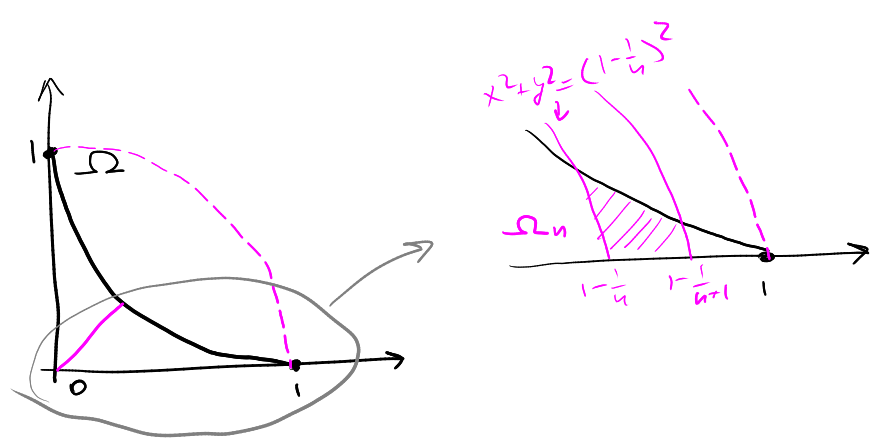
\includegraphics[scale=0.5]{6_2.png}
\end{center}
\end{task}
\begin{solution}
\[ \int_\Omega \frac{1}{|1 - x^2 - y^2|} dx dy = \sum_n \int_{\Omega_n} \asymp \sum \frac{1}{\left(\frac{1}{n}\right)^p}\cdot\frac{1}{n^{3.5}} \]
\end{solution}
\begin{task}
\end{task}
\section{Интеграл по поверхности}
\label{sec:orgedc4ad7}
\begin{center}
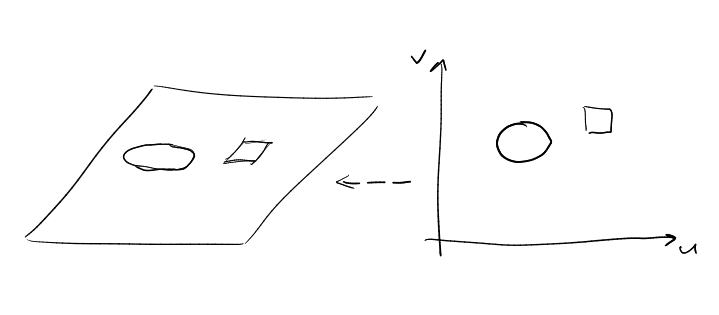
\includegraphics[scale=0.5]{6_3.png}
\end{center}
\[ \begin{array}{l} x(u, v) \\ y(u , v) \\ z(u, v) \end{array} \]
\[ S = \iint_\Omega |\overline{x}'_u\times\overline{x}'_v| du dv = \iint_\Omega \sqrt{EG - F^2} du dv \]
, где \(E = |\overline{x}_u'|^2 = x'_u^2 + y'_u^2 + z'_u^2\), \(F = (\overline{x}_u, \overline{x}_v) = x'_ux'_v + y'_uy'_b + z'_uz'_v\), \(G = |\overline{x}'_v|^2 = x'_v^2 + y'_v^2 + z'_v^2\)
\begin{task}
График \(z = z(x, y)\)
\end{task}
\begin{solution}
\[ \begin{array}{l} x = x \\ y = y \\ z = z(x, y) \end{array}\quad \begin{matrix} i \\ j \\ k \end{matrix} \begin{pmatrix} 1 \\ 0 \\ z'_x \end{pmatrix} \begin{pmatrix} 0 \\ 1 \\ z'_y \end{pmatrix} \quad \begin{matrix} -z'_x \\ -z'_y \\ 1 \end{matrix}\]
\[ S = \iint_\Omega \sqrt{1 + z'_x^2 + z'_y^2} dx dy \]
\end{solution}
\begin{task}
\[ x^2 + y^2 = a^2 \]
\[ az = xy \]
\end{task}
\begin{solution}
\[ S = \iint_{\begin{tikzpicture}
\draw (0, 0) circle[radius=0.2cm];
\end{tikzpicture}} \sqrt{1 + \frac{y^2}{a^2} + \frac{x^2}{a^2}}\,dx,dy = \left|\begin{matrix} x = a r \cos\varphi \\ y = a r \sin \varphi \end{matrix}\right. = \int\limits^1_0 dr \int\limits^{2\pi}_0 d\varphi \sqrt{1 + r^2}a^2 r = 2\pi a^2 (1 + r^2)^\frac{3}{2} \cdot \frac{1}{3} \bigg|^1_0 \]
\end{solution}
\begin{task}
\[ x^2 + y^2 = a^2 \]
\[ y^2 + z^2 = a^2 \]
\end{task}
\begin{solution}
\[ x = \sqrt{a^2 - z^2} \]
\[ x'_y = 0\quad x'_z = \frac{-z}{\sqrt{a^2 - z^2}} \]
\[ S = 4 \iint\limits_{y^2 + z^2 \le a^2} \sqrt{1 + \left(\frac{\partial x}{\partial y}\right)^2 + \left(\frac{\partial x}{\partial z}\right)^2}\, dy\, dz = 16 \int\limits_0^a dz \int\limits^{\sqrt{a^2 - z^2}}_0 \sqrt{1 + 0 + \left(-\frac{z}{x}\right)^2} dy = \]
\[ = 16 \int\limits^a_0 dz \int\limits^{\sqrt{a^2 - z^2}}_0 \frac{\sqrt{x^2 + z^2}}{x^2} dy = 16 a \int dz \int \frac{dy}{\sqrt{a^2 - z^2}} \]
\end{solution}

\begin{task}
\[ z^2 = 2xy\quad x + y = 1,\ x= 0,\ y = 0\]
\end{task}
\begin{solution}
\[ z = \sqrt{2xy}\quad \]
\[ \begin{matrix}
z'_x = \sqrt{\frac{y}{x}}\cdot \frac{1}{\sqrt{2}} \\
z'_y = \sqrt{\frac{x}{y}}\cdot \frac{1}{\sqrt{2}} \end{matrix }\]
\[ S = \iint \sqrt{1 + \frac{y}{2x} + \frac{x}{2y}}\,dx\,dy = \iint \sqrt{\frac{2xy + y^2 + x^2}{2xy}} = \iint \frac{x + y}{\sqrt{2}\sqrt{xy}} = \int\limits^1_0 dx \int\limits_0^{1 - x} \frac{\sqrt{x}}{\sqrt{2}}\cdot\frac{1}{\sqrt{y}} + \frac{1}{\sqrt{2}x}\cdot \sqrt{y} dy\]
\end{solution}

\begin{task}
\[ z = \sqrt{x^2 - y^2}\quad (x^2 + y^2)^2 = a^2(x^2 - y^2) \]
\end{task}
\begin{solution}
\[ \iint\limits_\Omega \sqrt{1 + \frac{x^2 + y^2}{x^2 - y^2}}\,dx\,dy = 4\sqrt{2} \iint \frac{x}{\sqrt{x^2 - y^2}}\,dx\,dy \]
\[ z'_x = \frac{x}{\sqrt{x^2 - y^2}}\quad z'_y = \frac{-y}{\sqrt{x^2 + y^2}} \]
\end{solution}
\end{document}
